%!TEX root = ../thesis.tex

\section{Стек протоколів OSI та TCP/IP}

OSI (Open Systems Interconnection) - модель, що була розроблена ISO для міжнародної стандартизації протоколів, що використовуються для комунікації між різними системами у 1995 році. Додамо, що основною ціллю було вирішення проблеми з'єднання відкритих систем, що є відкритими для комунікації із іншими системами. Наведемо табличку порівняння протоколів OSI та TCP/IP. 

\begin{figure}[ht]
        \centering
        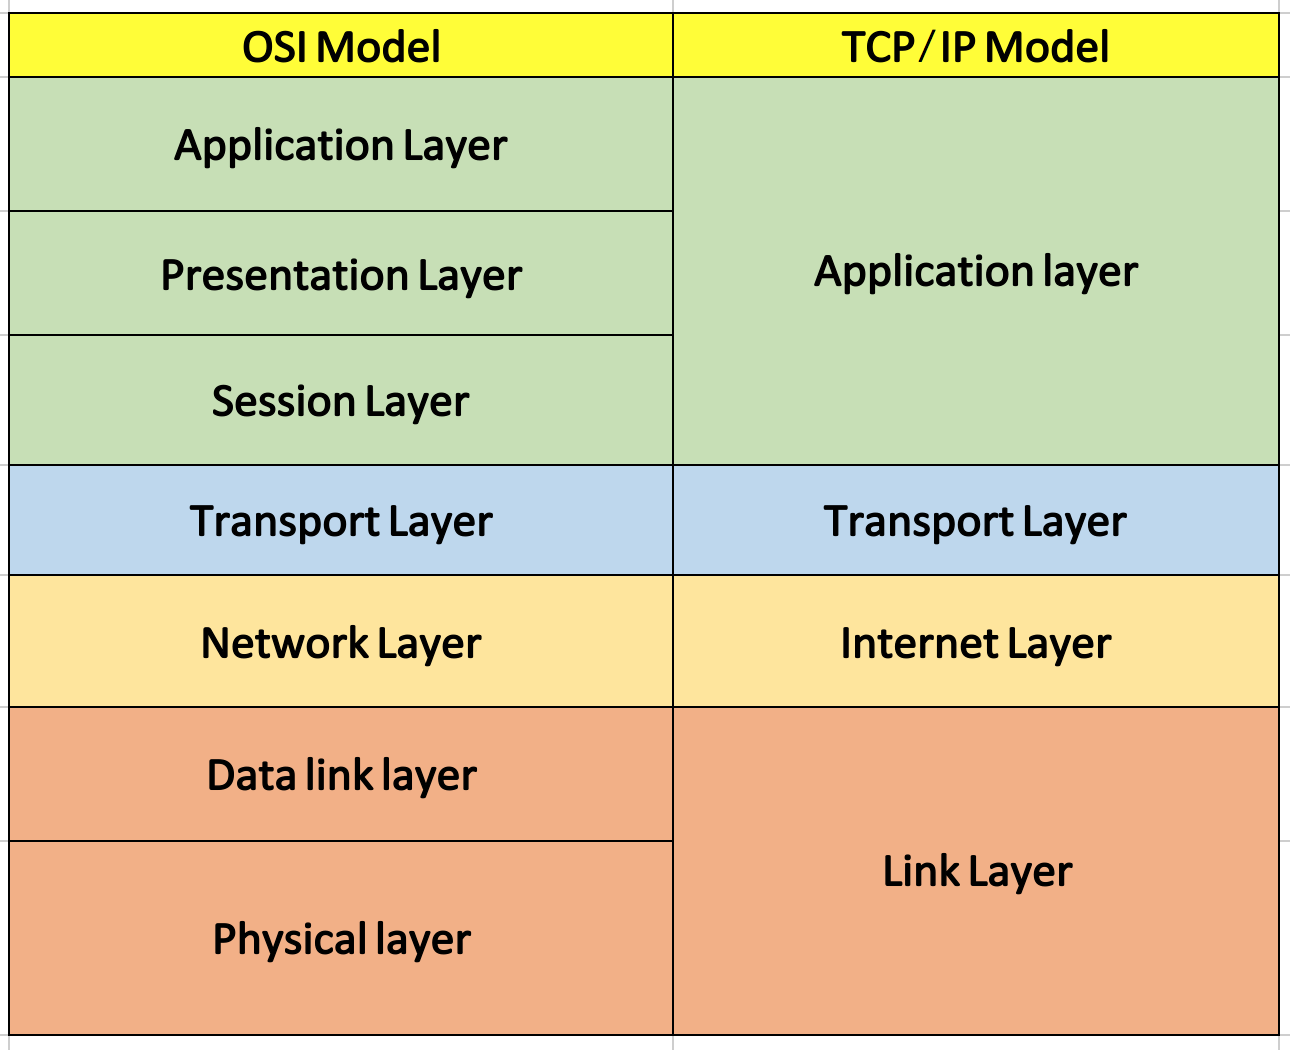
\includegraphics[scale=0.15]{../IMAGES/tcp_ip_osi.png}
        \caption{Набір протоколів TCP/IP у порівнянні із OSI.}
        \label{tcp_ip_protocols_suite}
\end{figure}

Модель OSI має 7 рівнів, тож опишімо їх:
\begin{itemize}
    \item \textbf{Фізичний рівень (Physical layer, L1)}
    Фізичний рівень відповідає за передачу необроблених бітів по каналу зв'язку. Проблеми проектування пов'язані з тим, щоб переконатися, що коли одна сторона надсилає 1 біт, інша сторона отримує його як 1 біт, а не як 0 біт. Типовими питаннями тут є: 
    \begin{itemize}
        \item Скільки вольт слід використовувати для представлення 1 і скільки для 0?
        \item Скільки наносекунд триває біт?
        \item Чи може передача відбуватися одночасно в обох напрямках?
        \item Як встановлюється початкове з'єднання встановлюється і як воно розривається?
        \item Коли обидві сторони закінчили комунікацію?
        \item Скільки контактів має мережевий роз'єм і для чого використовується кожен контакт?
    \end{itemize}
    Питання дизайну тут здебільшого стосуються механічних, електричних та часових інтерфейсів, а також фізичного середовища передачі даних, що лежить нижче фізичного рівня.

    \item \textbf{Канальний рівень (Data Link Layer, L2)}
    Основним завданням канального рівня є \textit{перетворення необробленої лінії передачі в лінію, яка виглядає вільною від невиявлених помилок передачі на мережевий рівень}. Він виконує це завдання, змушуючи відправника розбивати вхідні дані на кадри даних (зазвичай кілька сотень або кілька тисяч байт) і передавати ці кадри послідовно. 
    Якщо підсумувати, то саме тут вирішуються проблеми:
    \begin{itemize}
        \item підтвердження надісланих пакетів;
        \item утримання достатньо швидкого каналу у якому отримувач буде встигати отримувати та оброблювати повідомлення.
    \end{itemize}

    \item \textbf{Мережевий рівень (Network Layer, L3)}
    Мережевий рівень контролює роботу підмережі. Ключовим питанням проектування є \textit{визначення того, як пакети від джерела до місця призначення}.
    Якщо підсумувати, то саме тут вирішуються проблеми:
    \begin{itemize}
        \item визначення маршруту до потрібної адреси;
        \item контроль перевантажень (занадто великої кількості пакетів на вузлах).
    \end{itemize}

    \item \textbf{Транспортний рівень (Transport Layer, L4)}
    
    Транспортний рівень забезпечує зв'язок між двома процесами. Він гарантує, що дані, які надсилаються до місця призначення, повинні бути доставлені тому самому процесу, для якого вони призначені. Під процесом тут мається на увазі програма, що зв'язується із номером порту, що допомагає транспортному рівню ідентифікувати правильний процес, призначений для даних.

    Підсумуючи, транспортний рівень виконує наступні задачі із отриманими даними для передачі:
    \begin{enumerate}
        \item Сегментація - розбивка пакетів на атомарні величини для спрощення передачі даних.
        \item Контроль помилок - допомога іншому абоненту повністю зібрати повідомлення при наявності відсутніх чи пошкоджених сегментів при їх отриманні.
    \end{enumerate}

    У даний час на транспортному рівні існує два протоколи TCP (Transmission Control Protocol) та UDP (User Datagram Protocol). Їхню різницю буде зручно описати наступною таблицею.

    % і іще третій -- broadcast
    \begin{table}[ht]
    \label{tab:tcp_diff_udp}
    \begin{tabularx}{\textwidth}{X|X} 
	      \textbf{TCP} & \textbf{UDP} \\
        \hline
        Протокол керування передачею (TCP) є одним із основних протоколів набору протоколів Інтернету. В основному використовується для передачі веб-сторінок. & Протокол датаграм користувача (UDP) також є одним із найбільш використовуваних протоколів в Інтернеті. Протоколи UDP використовуються в багатьох системах, де стійке з’єднання не є головним пріоритетом і потрібна швидша передача даних та певна втрата даних є прийнятною. \\
        \hline
        Найважливішою особливістю TCP є:
            \begin{enumerate}
                \item Протокол орієнтований на підключення.
                \item Забезпечує зворотній зв’язок, коли пакет успішно отримано на іншому кінці, і це робить протокол TCP повільнішим.
                \item У TCP не може бути втрати даних.
            \end{enumerate}
             & Найважливішою особливістю UDP є:
            \begin{enumerate}
                \item Протокол без підключення.
                \item Дані передаються швидше, але дані можуть бути втрачені.
                \item У цьому не використовується механізм зворотного зв'язку.
            \end{enumerate} \\
    \end{tabularx}
        \caption{Різниця TCP та UDP між собою.}
    \end{table}

    \item \textbf{Сеансовий рівень (Session layer, L5)}
    Рівень сеансів дозволяє користувачам на різних машинах створювати сеанси між собою. Сеанси пропонують різноманітні сервіси:
    \begin{enumerate}
        \item контроль діалогу (відстеження того, чия черга передавати дані);
        \item управління токенами (запобігання спробам одночасного виконання критично важливих операцій);
        \item синхронізація (перевірка довгих передач, щоб дозволити їм продовжитися з того місця, де вони були після збою).
    \end{enumerate}

    \item \textbf{Рівень подання даних (Presentation Layer, L6)}
    На відміну від нижчих рівнів, які здебільшого займаються переміщенням бітів, \textit{рівень представлення займається синтаксисом та семантикою інформації, що передається}. Для того, щоб комп'ютери з різними представленнями даних могли взаємодіяти, структури даних, якими вони обмінюються різними представленнями даних, структури даних, якими вони обмінюються, можуть бути визначені в абстрактно, разом зі стандартним кодуванням, яке буде використовуватися «на дроті». 
    
    Рівень представлення керує цими абстрактними структурами даних і дозволяє визначати та обмінюватися структурами даних вищого рівня (наприклад, банківськими записами).

    Грубо кажучи, цей рівень буде займатися представленням картинок (JPEG, GIF, \dots), відео-аудіо (MPEG, Quicktime, \dots), а також шифруванням даних, коли під час передачі їх треба захистити.
    

    \item \textbf{Прикладний рівень (Application Layer, L7)}
    Прикладний рівень забезпечує зв'язок із процесами на рівні додатків, адже він включає протоколи, що використовують високорівневе API нижчих рівнів для взаємодії. 
    
    Прикладами протоколів, що фукнціонують на прикладному рівні є: HTTP - для передачі гіпертексту по мережі, FTP-клієнти -- протокол FTP для передачі файлів, поштові клієнти -- SMTP, службові пакети накшталт DHCP -- протокол призначення IP-адрес DHCP і так далі \dots. У більшості протоколи прикланого рівня асоціюються із конкретними клієнт-серверними додатками.    
\end{itemize}


\section{TCP/IP}

Стек протоколів TCP/IP(Transmission Control Protocol/Internet Protocol) є фундаментальною основою для комп'ютерних мереж, а саме - мережевою моделлю, що описує строгий процес предачі цифрових даних між абонентами. Сьогодні, оглядаючись на обсяг досліджень, що були пророблені для створення протоколів, здається чимось неймовірним, адже це все починалося створюватися для задоволення внутрішніх потреб із комунікації військових між собою.

Сама розробка TCP/IP була ініційована Департаментом Безпеки (DoD) США у далеких 1970 роках для з'єднання розрізнених і дуже різних локальних мереж. Згодом розробку і впроваження делегували різним підрядникам, що імплементували мережеву взаємодію для популярних операційних систем IBM подібних та UNIX. Формально цей стек протоколів є описаний у такому стандарті RFC 9293, але вони не обмежуються на одному, є ще підпротоколи, які дозволяють у якомусь сенсі <<розмежувати>> зону відповідальності кожного із них.

Згадаємо, що протоколи є наборами правил для форматів повідомлень і процедур, які дозволяють машинам і прикладним програмам обмінюватися інформацією. Тож ці правила повинні виконуватися кожною машиною, що бере участь у зв’язку, щоб приймаючий хост міг зрозуміти повідомлення. Набір протоколів TCP/IP можна зрозуміти з точки зору рівнів (або рівнів). Формально ці рівні можна побачити у таких стандартах: RFC 1122 та RFC 1123.

Відповідно до \ref{tcp_ip_protocols_suite} можна побачити, що OSI модель можна перетворити у TCP/IP модель об'єднавши певні рівні між собою.

Також додамо цікаву репрезентацію мережевих рівнів, а саме як вони врапляться один в один та навпаки розкриваються для забезпечення поставленої задачі.

\begin{figure}[ht]
\centering
    \begin{subfigure}[b]{0.5\textwidth}    
        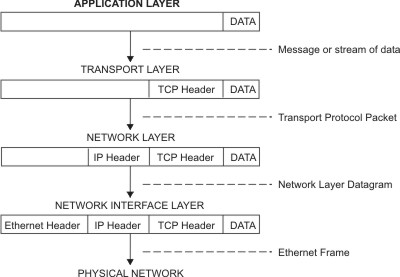
\includegraphics[scale=1.9]{../IMAGES/tcp_ip_layers_app_host.jpg}
        \caption{}
        % обратите внимание на знак % после \end{subfigure} и 
        % отсутствие пустых строк и разделителей после \end{subfigure}
        % -- это сливает в одну строку подфигуры
    \end{subfigure}%
    \begin{subfigure}[b]{0.5\textwidth}
        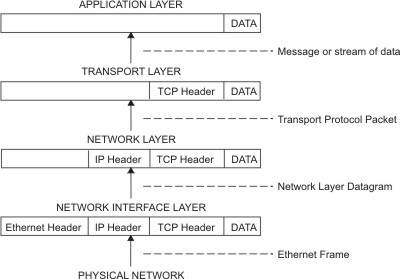
\includegraphics[scale=1.9]{../IMAGES/tcp_ip_layers_host_app.jpg}
        \caption{}
    \end{subfigure}
 
    \caption{{Розбивка пакетів TCP/IP із прикладного рівня до найнижчих і навпаки.}}
    \label{fig_sudak}
\end{figure}


\begin{description}
        \item[Чому у вижитку у нас є і OSI та TCP/IP?] \hfill \\

        OSI та TCP/IP мають у собі багато спільного, обоє засновані на коцепції розрізнених незалежних протоколів. Також мають багато спільного, до прикладу, мають однакові моделі транспортного рівня, яка дає можливість забезпечення незалежного від мережі транспортного обслуговування процесів, що бажають спілкуватися. Не зважаючи на певні схожості, все ж таки вони мають у собі різницю.
        \begin{enumerate}
            \item Погане проектування. Вибір семи рівнів у OSI був більше політичним кроком чим технічним, адже два рівні (сесійний та представлення даних) є майже пустими, коли (канальний рівень та мережевий) переповнені обов'язками. 
            \item Час випуску. TCP/IP модель була запущенна у використання задовго до появи OSI формального стандарту. Тобто, коли університети, компанії, уже наповну досліджували та використовували першу модель, то друга ще розроблялася і вийшла запізно. Мало того, більшість не бажала підтримувати ще другий стек протоколів за відсутності початкових пропозицій по імплементації, тощо.
        \end{enumerate}
        Тож, хоча стандартизація та широке впровадження OSI було провалене, але він всеодно залишився як можлива модель, і має певне використання для пояснення певних думок у суспільстві. 
    \end{description}

\section{SSL vs TLS}

SSL та TLS грубо кажучи можна охарактеризувати як одна і та ж технологія, тільки із використанням різних назв. SSL або (Secure Socket Layer) версія 1.0 була розроблена у 1994 році Netscape. У результаті їх було всього 3 версії, а уже із розробкою та використанням 3 версії було представлено TLS 1.0. TLS або (Transport Layer Security) є фактично версією SSL 3.0, але є достатньо зміненим для того, щоб вважатися <<SSL 3.1>>. Перейменування було здійснене із метою зміною назви стандарту, щоб не було колізій із уже опублікованим стандартом. 

Протокол TLS (SSL) знаходиться між транспортними та прикладними рівнями. Конкретне місце показане на схемі.

\begin{figure}[ht]
        \centering
        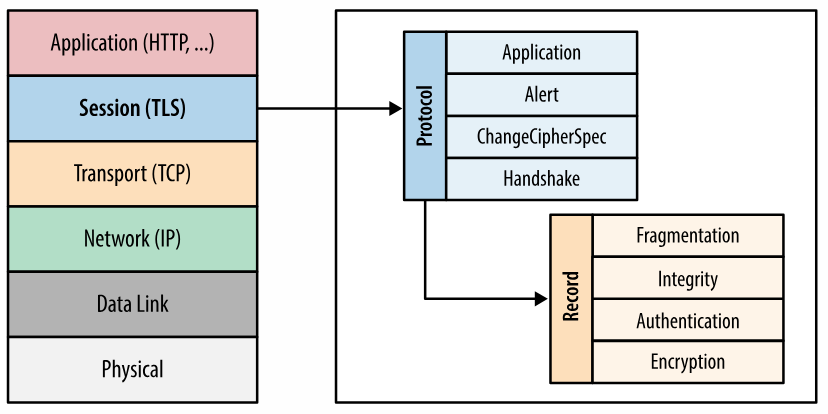
\includegraphics[scale=0.35]{../IMAGES/tls_oreally.png}
        \label{tls_oreally}
\end{figure}

Цей протокол призначений для надання трьох основних послуг для всіх додатків, що працюють над ним, а саме:
\begin{enumerate}
    \item \textbf{\textit{автентифікація}} -- механізм перевірки дійсності наданих ідентифікаційних даних та перевірки справжньості серверної частини. Додамо, що користувач не обов'язково повинен у TLS бути автентифікованим;
    \item \textbf{\textit{конфіденційність}} -- механізм для приховування того, що надсилається від одного хоста до іншого. Мається на увазі, що дані, надіслані по каналу після встановлення зв'язку видимі лише для кінцевих абонентів (endpoints). TLS не приховує довжину даних, які він передає, хоча кінцеві точки можуть доповнювати TLS записів, щоб приховати довжину та покращити захист від методи аналізу трафіку.
    \item \textbf{\textit{цілісність}} -- механізм виявлення фальсифікації та підробки повідомлень. Мається на увазі, що дані, надіслані через канал після встановлення зв'язку, не можуть бути зміненими зловмисниками без виявлення цього факту.
\end{enumerate}

На відміну від цих властивостей, TLS складається із двох основних частин: 

\begin{itemize}
    \item Протокол рукостискання або (handshake protocol) автентифікує сторони, що спілкуються, узгоджує криптографічні режими та параметрів і встановлює спільний ключовий матеріал. Протокол рукостискання розроблений таким чином, щоб протистояти втручанню; активний зловмисник не повинен мати змоги змусити учасників рукостискання узгодити інші параметри, ніж якщо з'єднання не було атаковано.
    \item Протокол записів (record protocol) використовує параметри, встановлені протоколом рукостискання для захисту трафіку між взаємодіючими одноранговими системами. Протокол записів розділяє трафік на серію записів, кожен з яких незалежно захищений за допомогою ключів трафіку.
\end{itemize}

Надалі ми розглянемо лише протокол рокостискання, а протокол обміну записами можна буде розглянути у RFC 8446.

\subsection{SSL, TLS версії}

\begin{figure}[ht]
        \centering
        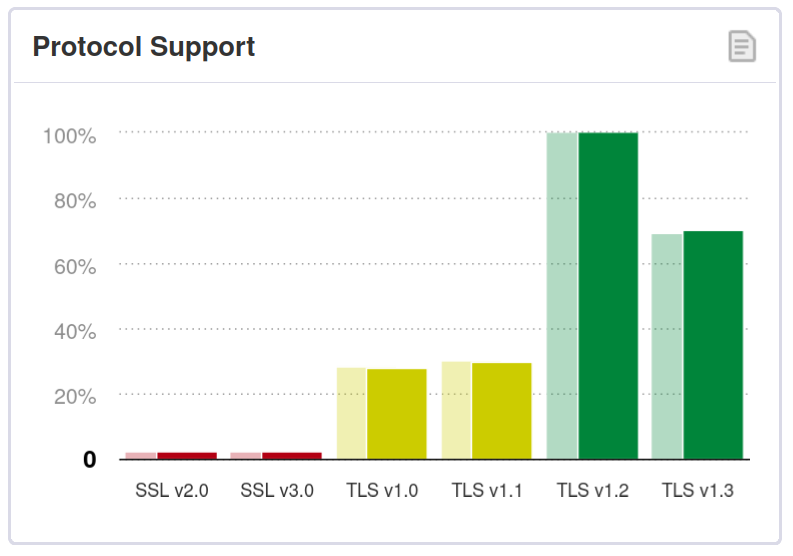
\includegraphics[scale=0.35]{../IMAGES/ssl_support.png}
        \caption{Підтримка версій SSL у Інтернеті станом на квітень 2024 року.}
        \label{ssl_support}
\end{figure}

Коротко підсумуємо послідовність випуску версій SSL та TLS разом із коротким описом:
\begin{enumerate}
    \item SSL 1.0 так і ніколи не була публічно випущена через деякі серйозні недоліки безпеки.
    
    \item SSL 2.0 було опубліковано Netscape у 1995 році. Головними претензіями до цієї версії були структурні недоліки у самому протоколі обміну повідомленнями.
    
    \item SSL 3.0 було опубліковано у стандарті \texttt{IETF RFC 2246} у 1996 році. Цього разу SSL спіткав повний редизайн протоколу, а саме за допомогою таких функцій, як 128-бітове шифрування, ланцюжки сертифікатів, гнучкі протоколи обміну ключами, стиснення даних і зворотна сумісність із SSL 2.0. Із вразливостей протокол мав POODLE (Padding Oracle On Downgraded Legacy Encryption) вразливість, яка дозволяє зловмисникам використовувати недоліки заповнення в режимі CBC, потенційно дешифруючи конфіденційні дані.
    
    \item TLS 1.0 був визначений у RFC 2246 у січні 1999 року та є оновленням SSL 3.0 з відмінностями у функціях отримання ключів, використанні HMAC, іншому формуванні повідомлень оповіщення та попередження, підтримці DSS/DH, що робить його несумісним із SSL 3.0. Додамо, що зміни які були внесені сюди було достатньо для того, щоб вважати їх окремими протоколами.
    
    \item TLS 1.1 був представлений у 2006 році, що покращив TLS 1.0, а саме додавши захист від CBC-атак за допомогою явних векторів ініціалізації, уточнення оброблення помилок і підвищення стійкість до певних cipher-block chaining уразливостей.
    
    \item TLS 1.2 був опублікований 2008 року у стандарті RFC 5246, що удосконалив TLS 1.1, а саме за допомогою:
    \begin{enumerate}
        \item посилення вимог для виконання протоколу;
        \item виправлення атак Блейхенбахера та Дліма у структурі протоколу;
        \item зміни застарілих алгоритмів на більш нові.
    \end{enumerate}

    \item TLS 1.3 на даний час є найдосконалішою версією протоколу, що була опублікована 2018 року у стандарті RFC 8446. Було реалізовано:
    \begin{enumerate}
        \item шифрування після першого повідомлення ServerHello;
        \item оновлення списку симетричних алгоритмів;
        \item покращення структури протоколу та зміни інших параметрів алгоритмів.
    \end{enumerate}
\end{enumerate}

\subsection{TLS 1.2}

Опишімо алгоритм налагодження захищенного спілкування між абонентами для версії TLS 1.2.

Спершу зв'язок за допомогою SSL починається з обміну інформацією між клієнтом і сервером. Цей обмін інформацією називається \texttt{рукостисканням SSL}. Рукостискання SSL складається з наступних етапів:
\begin{enumerate}
    \item \textbf{Узгодження набору шифрів}. 
    
    Сеанс SSL починається з узгодження між клієнтом і сервером про те, який набір шифрів вони будуть використовувати. Набором шифрів будемо називати набір криптографічних алгоритмів і розмірів ключів, які комп'ютер може використовувати для шифрування даних. Набір шифрів містить інформацію про алгоритми обміну відкритими ключами або алгоритми узгодження ключів, а також криптографічні хеш-функції. Клієнт повідомляє серверу, які набори шифрів йому доступні, а сервер вибирає найкращий взаємоприйнятний набір шифрів.
    
    \item \textbf{Перевірка автентичності сервера (опціональна).}
    
    В SSL етап автентифікації не є обов'язковим, але в випадку транзакції електронної комерції через Інтернет клієнт, як правило, хоче автентифікувати сервер. Автентифікація сервера дозволяє клієнту бути впевненим, що сервер представляє саме ту організацію, яку, на думку клієнта, він представляє.
    
    Щоб довести, що сервер належить саме тій організації, за яку він себе видає, сервер надає клієнту свій сертифікат відкритого ключа. Якщо цей сертифікат дійсний, то клієнт може бути впевнений в ідентичності сервера.

    Клієнт і сервер обмінюються інформацією, яка дозволяє їм узгодити один і той же секретний ключ. До прикладу, в RSA клієнт використовує відкритий ключ сервера, отриманий з сертифіката відкритого ключа, для шифрування інформації секретного ключа. Клієнт надсилає зашифровану інформацію про секретний ключ на сервер. Тільки сервер може розшифрувати це повідомлення, оскільки для цього потрібен закритий ключ сервера.
    
    \item \textbf{Узгодження механізмів шифрування}
    
    Тепер і клієнт, і сервер мають доступ до одного і того ж секретного ключа. З кожним повідомленням вони використовують криптографічну хеш-функцію, обрану на першому кроці рукостискання, і спільну секретну інформацію, щоб обчислити HMAC, який вони додають до повідомлення. Потім вони використовують секретний ключ і алгоритм секретного ключа, узгоджений на першому етапі рукостискання, для шифрування захищених даних і HMAC. Тепер клієнт і сервер можуть безпечно спілкуватися, використовуючи свої зашифровані та хешовані дані.
\end{enumerate}

Тепер розгляньмо наступну діаграму, що показує послідовність повідомлень, що підлягають для обміну для SSL рукостискання. Додамо, що повідомлення, що помічені як \texttt{(Optional)} будуть надіслані лише за вимогою користувача чи сервера.

\begin{figure}[ht]
        \centering
        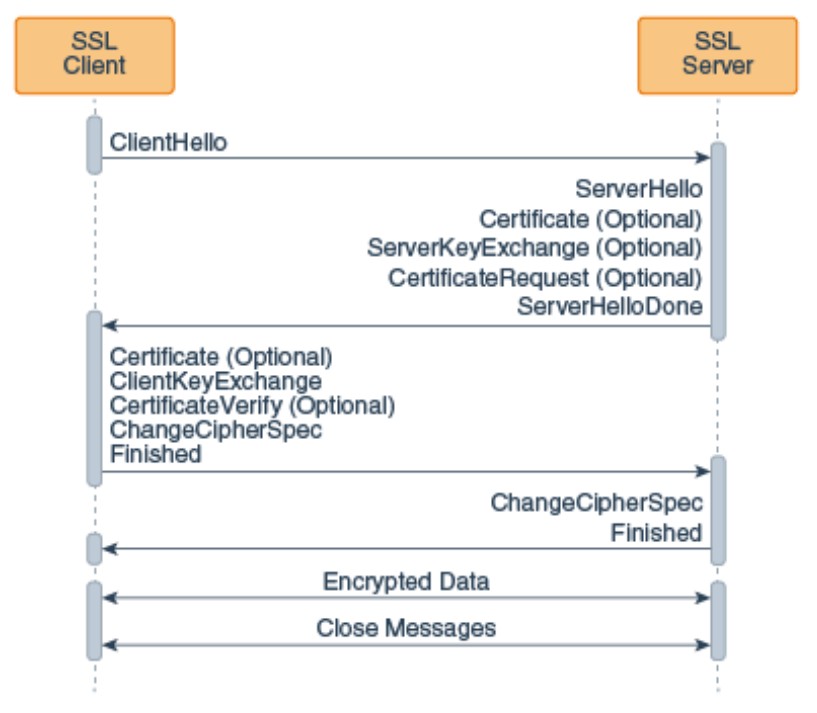
\includegraphics[scale=0.35]{../IMAGES/tls_1_2.png}
        \label{tls_1_2}
\end{figure}

Надалі будемо використовувати позначення \texttt{C} $\longrightarrow$ / $\longleftarrow$ / $\longleftrightarrow$ \texttt{S}, що у свою чергу позначає порядок надсилання даних від клієнта (\texttt{C}) до сервера (\texttt{S}).
\begin{enumerate}
    \item[1. \texttt{С} $\longrightarrow$ \texttt{S}] \textbf{Client hello.} Клієнт надсилає серверу інформацію, включаючи найвищу версію SSL, яку він підтримує, і список наборів шифрів, які він підтримує. Інформація про набір шифрів включає криптографічні алгоритми та розміри ключів.
    \item[2. \texttt{С} $\longleftarrow$ \texttt{S}] \textbf{Server hello.} Сервер вибирає найвищу версію SSL і найкращий набір алгоритмів шифрування, які підтримуються клієнтом і сервером та надсилає цю інформацію клієнту.
    \item[3. \texttt{С} $\longleftarrow$ \texttt{S}] (Опціонально) \textbf{Certificate.} Сервер надсилає клієнту сертифікат або ланцюжок сертифікатів. Ланцюжок сертифікатів зазвичай починається з сертифіката відкритого ключа сервера і закінчується кореневим сертифікатом центру сертифікації. Це повідомлення є необов'язковим, але використовується щоразу, коли потрібна автентифікація сервера.
    \item[4. \texttt{С} $\longleftarrow$ \texttt{S}] (Опціонально) \textbf{Certificate request.} Якщо сервер повинен автентифікувати клієнта, він надсилає клієнту запит на отримання сертифіката. Загалом у Інтернет додатках це повідомлення надсилається рідко.
    \item[5. \texttt{С} $\longleftarrow$ \texttt{S}] (Опціонально) \textbf{Server key exchange.} Сервер надсилає клієнту повідомлення із ключем сервера для обміну ними, якщо інформації про відкритий ключ із сертифіката недостатньо для обміну ключами. До прикладу, у наборах шифрів на основі Diffie-Hellman (DH) це повідомлення містить відкритий ключ DH сервера.
    \item[6. \texttt{С} $\longleftarrow$ \texttt{S}] \textbf{Server hello done.} Сервер повідомляє клієнту, що він закінчив обробку початкових повідомлень для рукостискання.
    \item[7. \texttt{С} $\longrightarrow$ \texttt{S}] (Опціонально) \textbf{Certificate.} Якщо сервер запитує сертифікат у клієнта, клієнт надсилає свій ланцюжок сертифікатів так само, як це робив раніше сервер.
    \item[8. \texttt{С} $\longrightarrow$ \texttt{S}] \textbf{Client key exchange.} Клієнт генерує інформацію, яка використовується для створення ключа для симетричного шифрування. Для RSA клієнт шифрує цю ключову інформацію за допомогою відкритого ключа сервера і надсилає її серверу. Для наборів шифрування на основі DH це повідомлення містить відкритий ключ DH клієнта.
    \item[9. \texttt{С} $\longrightarrow$ \texttt{S}] (Опціонально) \textbf{Certificate verify.} Це повідомлення надсилається клієнтом, коли клієнт надає сертифікат, як описано вище. Його мета - дозволити серверу завершити процес автентифікації клієнта. Як використовується це повідомлення, клієнт повинен надіслати інформацію, яку він підписує цифровим підписом із викоритстанням узгодженої геш фукнції. У свою чергу сервер повинен розшифрувати дані за допомогою відкритого ключа та верифікувати їх.
    \item[10. \texttt{С} $\longrightarrow$ \texttt{S}] \textbf{Change cipher spec.} Клієнт надсилає серверу повідомлення про перехід у зашифрований режим.
    \item[11. \texttt{С} $\longrightarrow$ \texttt{S}] \textbf{Finished.} Клієнт повідомляє серверу, що він готовий до початку безпечної передачі даних.
    \item[12. \texttt{С} $\longleftarrow$ \texttt{S}] \textbf{Change cipher spec.} Сервер надсилає клієнту повідомлення про перехід у зашифрований режим.
    \item[13. \texttt{С} $\longleftarrow$ \texttt{S}] \textbf{Finished.} Сервер повідомляє клієнту, що він готовий до початку безпечної передачі даних. Це кінець рукостискання SSL.
    \item[14. \texttt{С} $\longleftrightarrow$ \texttt{S}] \textbf{Encrypted data.} Клієнт і сервер обмінюються даними за допомогою симетричного алгоритму шифрування і  геш функції, що були узгоджені під час \texttt{(Client/Server) hello}, а також за допомогою секретного ключа, який клієнт відправив серверу під час обміну клієнтськими ключами. Рукостискання за потреби може бути повторно узгоджене в цей час.
    \item[15. \texttt{С} $\longleftrightarrow$ \texttt{S}] \textbf{Close messages.} В кінці з'єднання кожна сторона може надіслати спеціальні повідомлення про закриття з'єднання або просто розірвати його.
\end{enumerate}


\subsection{TLS 1.3}

\begin{figure}[ht]
        \centering
        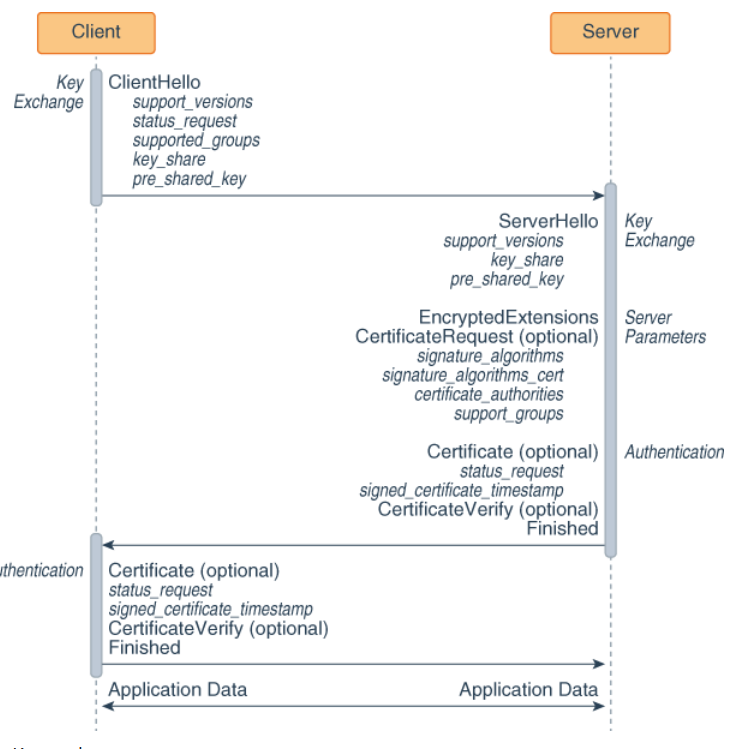
\includegraphics[scale=0.35]{../IMAGES/tls_1_3.png}
        \label{tls_1_3}
\end{figure}

TLS 1.3 у свою чергу був покращений у кількості надсилань повідомлень у обидва боки (round-trip). Із двох, що було у TLS 1.2, скоротилося до одного. Розгляньмо цей протокол.

Цього разу рукостискання складається з трьох етапів:
\begin{enumerate}
    \item \textbf{Обмін ключами}. На цьому етапі точно так само як і у TLS 1.2 встановлюється спільний ключ.
    \item \textbf{Параметри сервера}. На цьому етапі встановлюються інші параметри рукостискання разом із параметрами сервера, що були виставлені.
    \item \textbf{Автентифікація}. На цьому етапі виконується автентифікація сервера і клієнта за потреби, а також підтвердження ключа та цілісності рукостискання.
\end{enumerate}


Розгляньмо тепер сам обмін ключами.

\begin{enumerate}
    \item[1. \texttt{С} $\longrightarrow$ \texttt{S}] \textbf{Обмін ключами.} 
    \begin{enumerate}
        \item Клієнт надсилає серверу повідомлення \textbf{ClientHello}.
        \item Сервер обробляє повідомлення \textbf{ClientHello} і визначає відповідні криптографічні параметри для з'єднання. Потім він відповідає власним повідомленням \textbf{ServerHello}, в якому вказує узгоджені параметри з'єднання. Для TLS 1.3 повідомлення \textbf{ServerHello} визначає тільки ключ і параметри шифрування. Інші параметри рукостискання можуть бути визначені пізніше.
    \end{enumerate}
        
    \item[2. \texttt{С} $\longleftarrow$ \texttt{S}] \textbf{Параметри сервера.} Сервер надсилає два повідомлення для встановлення параметрів сервера.

    \begin{enumerate}
        \item \textbf{EncryptedExtensions}: Це повідомлення містить відповіді на розширення \textbf{ClientHello}, які не потрібні для визначення криптографічних параметрів, окрім тих, які є специфічними для окремих сертифікатів.
        \item \textbf{CertificateRequest} (опціонально): Якщо потрібна автентифікація клієнта на основі сертифіката, то сервер надсилає це повідомлення, яке містить бажані параметри для цього сертифіката. Уточнимо, що це повідомлення не надсилається, якщо автентифікація клієнта не потрібна.
    \end{enumerate}
    
    \item[3. \texttt{С} $\longrightarrow$ \texttt{S}] \textbf{Автентифікація}. 
    \begin{enumerate}
        \item 
              Сервер надсилає наступні повідомлення для автентифікації.
              \begin{itemize}
                \item \textbf{Certificate} (опціонально). Це повідомлення містить сертифікат автентифікації та будь-які інші підтримуючі сертифікати у ланцюжку сертифікатів. Це повідомлення не надсилається, якщо сервер не виконує автентифікацію за допомогою сертифіката. Примітка: Повідомлення Certificate може містити відкритий ключ замість сертифіката.
                \item \textbf{CertificateVerify} (опціонально). Повідомлення містить підпис по всьому рукостисканню з використанням закритого ключа, що відповідає відкритому ключу в повідомленні про сертифікат. Це повідомлення не передається, якщо сервер не автентифікується за допомогою сертифіката.
                \item \textbf{Finish}. Надсилається MAC-код (Message Authentication Code) для всього рукостискання.
              \end{itemize}
              
        \item Клієнт відповідає власними повідомленнями \textbf{Certificate}, \textbf{CertificateVerify} і \textbf{Finished}. 
        
        \begin{itemize}
            \item Повідомлення \textbf{Certificate} не надсилається, якщо сервер не надіслав повідомлення \textbf{CertificateRequest}.
            \item Повідомлення \textbf{CertificateVerify} не надсилається, якщо клієнт не автентифікується за допомогою сертифіката.
        \end{itemize}
    \end{enumerate}
    
    \item[4. \texttt{С} $\longleftrightarrow$ \texttt{S}] \textbf{Encrypted data.} Клієнт і сервер можуть безпечно надсилати дані програми один одному.
   
\end{enumerate}

\section{Ciphersuits}

У цьому розділі розглянемо доступні алгоритми для шифрування трафіку у TLS. Спочатку покажемо на прикладі актуального TLS 1.3 доступні збірки алгоритмів \ref{tls_1_3_ciphersuits}.

\begin{figure}[ht]
        \centering
        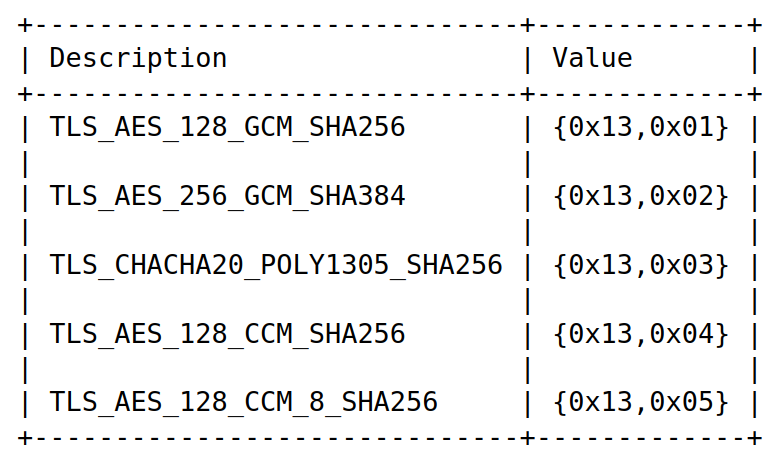
\includegraphics[scale=0.35]{../IMAGES/ciphersuits.png}
        \caption{Підтримка можливих алгоритмів шифрування у TLS $1.3$. Взято із додатку \texttt{B.4} до RFC 8446}.
        \label{tls_1_3_ciphersuits}
\end{figure}

У TLS 1.3 було значно зменшено кількість підтримуваних наборів ширфів із 37 у TLS 1.2 до 5. Як результат, було видалено незахищені та слабкі набори шифрів, залишено більш безпечні та сучасні набори шифрів. Додамо, що дизайн TLS 1.3 змінив концепцію набору шифрів. Він відокремлює механізми автентифікації та обміну ключами від алгоритму захисту записів і хешу, який використовується як з функцією отримання ключа(HKDF), так і з кодом автентифікації повідомлень рукостискання (MAC). Тобто оголошеня можливих алгоритмів для цифрового підпису, що підтримує користувач буде оголошене у окремому полі ServerHello повідомленні.

Нова конвенція іменування набору шифрів має вигляд \texttt{TLS\_<AEAD>\_<Hash>}, де алгоритм хешування використовується для нової визначеної функції отримання ключа у HKDF в TLS 1.3 і генерації MAC на етапі рукостискання. Набори шифрів, визначені протоколом TLS 1.3 є наступними \ref{tls_1_3_ciphersuits}.

Тепер треба пояснити суть криптографічних алгоритмів, що використовуються у даній нотації.
\begin{itemize}
    \item AEAD або (Authenticated Encryption with Associated Data) --  це форма шифрування, яка на додачу до забезпечення конфіденційності відкритого тексту, що є зашифрованим, забезпечує спосіб перевірки його цілісності та автентичності. У більшості це досягається за допомогою режимів блокового шифрування GCM та CCM, що генерують MAC, який можна автентифікувати у результаті за допомгою певних вхідних векторів ініацілізації, що були оголошені у одному пакеті та наперед узгоджені обома сторонами.
    \item Hash -- алгоритми гешування, що дозволяють потім використовувати їх у алгоритмах HKDF (Hash Key Deviation Function), тобто для того, щоб можна було безпечно отримувати різні ключі із попередньо ініацілізованого алгоритму.
\end{itemize}

\section{Сертифікати X.509}

Сертифікати, насамперед, у контексті формування TLS рукостискання використовуються для автентифікації користувачів чи серверів. Вони усвою чергу повинні бути сформовані відповідно X.509 PKI стандарту, що описаний у RFC 5280.

\begin{figure}[ht]
        \centering
        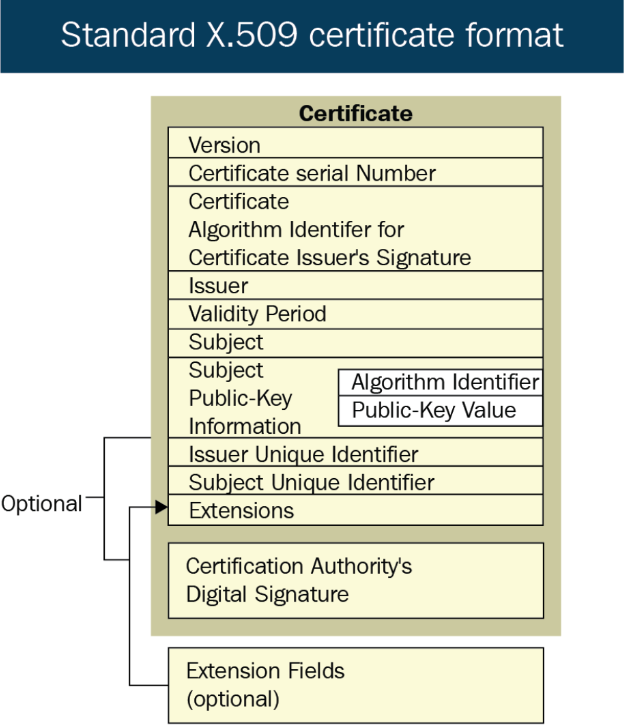
\includegraphics[scale=0.35]{../IMAGES/x_509_standard.png}
        \label{x_509}
\end{figure}

Загалом сертифікати у такому форматі мають бути створені за допомогою кодування ASN.1, яке може  складатися із наступних полів, що продемонстровані на картинці \ref{x_509}. Опишемо деякі із них.
\begin{itemize}
    \item \textbf{Version} - ціле число, яке визначає номер версії сертифіката.
    \item \textbf{Certificate serial Number} - ціле число, яке представляє унікальний номер для кожного сертифіката, виданого центром сертифікації (або CA).
    \item \textbf{Сertificate Algorithm OID for CA sign} - ідентифікатор криптографічного алгоритму, який використовується ЦС для підпису сертифіката. Значення включає як ідентифікатор алгоритму, так і будь-які додаткові параметри, які використовуються цим алгоритмом, якщо такі є.
    \item \textbf{Issuer} - розрізнюване ім’я (або Distinguished Name) ЦС, що видає сертифікат.
    \item \textbf{Validity period} - включний період часу, протягом якого дійсний сертифікат.
    \item \textbf{Subject} - визначне ім'я (DN) суб'єкта сертифіката.
    \item \textbf{Subject Pub-k} - відкритий ключ, яким володіє суб’єкт сертифіката.
    \item \textbf{Issuer Unique Identifier} - унікальний ідентифікатор, який представляє ЦС видачі, як визначено ЦС видачі.
    \item \textbf{Subject Unique Identifier} - унікальний ідентифікатор, який представляє суб’єкт сертифіката, як визначено центром сертифікації.
    \item \textbf{Extensions} - набір стандартних і специфічних для Інтернету розширень сертифікатів. До прикладу, сертифікат може бути обмежений лише для автентифікації абонента, лише для підпису чи лише для шифрування. Усі додакові розширення до сертифікату можна подивися у документації. 
    \item \textbf{Certificate Authority Digital Signature} - підпис ЦС, що підтверджує видачу сертифіката.
\end{itemize}

\begin{figure}[ht]
        \centering
        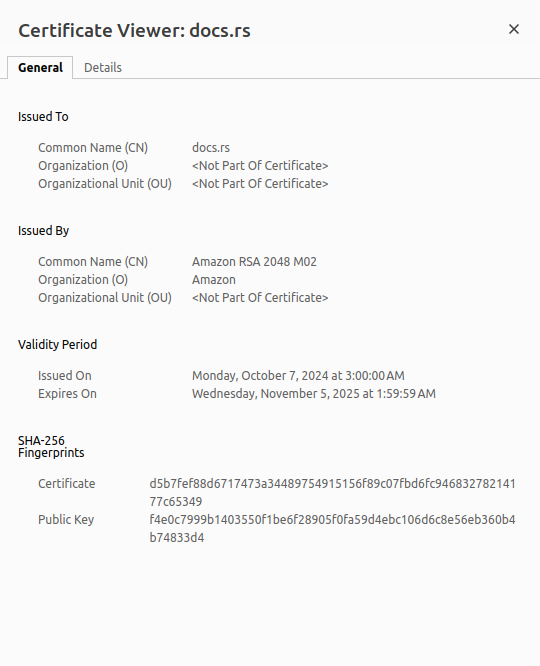
\includegraphics[scale=0.35]{../IMAGES/certificate_example.png}
        \label{certificate_example}
        \caption{Приклад сертифікату, що є доступним для веб сторінки \texttt{doc.rs}.}
\end{figure}

\subsection{Інфраструктура відкритих ключів}

 Не дарма у стерифікатах X.509 стандарту передбачено поле для підпису ЦС, адже сертифікати просто так не можуть існувати. Їх обов'язково треба підверджувати довіреною особою, у даному випадку це є Центри Сертифікації і навкого цього побудована ціла інфраструктура, що звесться PKI або Public Key Insfrastructure. PKI - це технологія, що забезпечує 
 \begin{itemize}
     \item призначення;
     \item розпізнавання;
     \item перевірку користувачів;
 \end{itemize} 
 за допомогою цифрових сертифікатів, що використовуються для забезпечення надійного та безпечного цифрового зв'язку.

 Основними компонентами PKI є:
 \begin{itemize}
     \item \textbf{Центр сетифікації} - довірена організація, відповідальна за видачу, зберігання та підпис цифрових сертифікатів. Центри сертифікації використовують свій власний закритий ключ для підпису цифрових сертифікатів, який можна перевірити за допомогою відкритого ключа, який є у доступі.
     \item \textbf{Підлеглий ЦС} (або орган реєстрації) - центр сертифікації, що відповідає за перевірку особи користувача або пристрою, що запитує цифровий сертифікат чи намагається його створити.
     \item \textbf{База даних сертифікатів} - доступна база даних, що зберігає окремі цифрові сертифікати, включаючи метадані, як-от період дії сертифіката.
     \item \textbf{Політика керування сертифікатами} - загальнодоступна політика з детальним описом процедур і стандартів PKI. Треті сторони також можуть використовувати політику сертифікатів для отримання доступу до PKI.
     \item \textbf{Користувачі} - кінцеві суб'єкти, що кристуються послугами.
 \end{itemize}

У PKI, окрім, вищезгаданих функцій разом із видачею сертифікатів існує функція перевірки сертифікатів на дійсність та актуальність. Для цього у політиках керування сертифікатами існують спеціальні CRL (Certificate Revocation Lists) списки відкликаних сертифікатів та OSCP (Online Certificate Status Protocol) - запити на отримання статусу сертифіката.

Саме у контексті TLS варто ввести таке поняття як ланцюг довіри. Ланцюг довіри – це модель безпеки, яка використовується в цифрових сертифікатах для перевірки легітимності сертифіката, наданого веб-сайтом або службою. Він ґрунтується на ієрархічній структурі, де кожен сертифікат у ланцюжку підписується вищим, надійним органом, доки він не досягне кореневого сертифіката, якому система або браузер буде довіряти. 

\begin{figure}[ht]
        \centering
        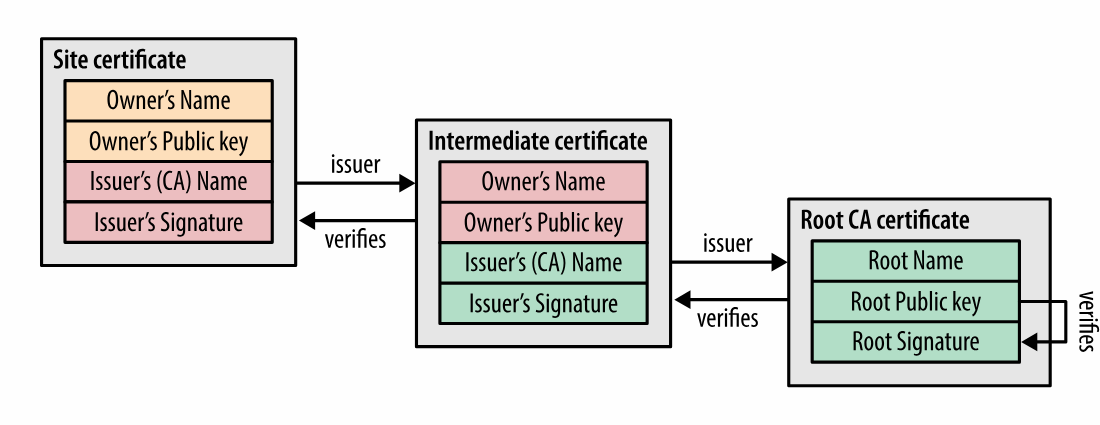
\includegraphics[scale=0.35]{../IMAGES/certificate_chain.png}
        \label{certificate_chain}
\end{figure}

Тобто під час побудови ланцюжка довіри необхідно перевіряти актуальність кожного довірчого вузла. За допомогою вище згаданих фукнцій PKI, публікація CRL списківі є дуже важливою, адже саме по ній треба орієнтуватися чи сертифікат не є відкликаним. CRL списки у свою чергу є простим набором серійних номерів сертифікатів, що були відкликані, тож кожен користувач може перевірити будь-який сертифікат на актуальність, але тут постає проблема у ефективному використанні ресурсів. Тож кожен раз викачувати файл із числами і перевіряти чи є певний номер у списку не є раціональним. Щоб вирішити цю проблему було вирішено створити OCSP запити, що будуть динамічно відповідати клієнту про статус сертифіка(-та/-ів).


OSCP запити є Інтернет протоколом, що використовується для отримання статусу відкликання сертифікату. В основному цей протокол описаний у RFC 6960. OSCP сервер може повернути підписану відповідь, що вказує у якому стані преебуває той чи інший сертифікат: good(сертифікат актуальний), revoked(сертифікат відкликаний), unknown(невідомо жодної інформації про сертифікат). Якщо він не може обробити запит, він може повернути код помилки.

\section{Вразливості TLS}

\begin{itemize}
\item \textbf{Атака переузгодження}

    \begin{figure}[ht]
        \centering
        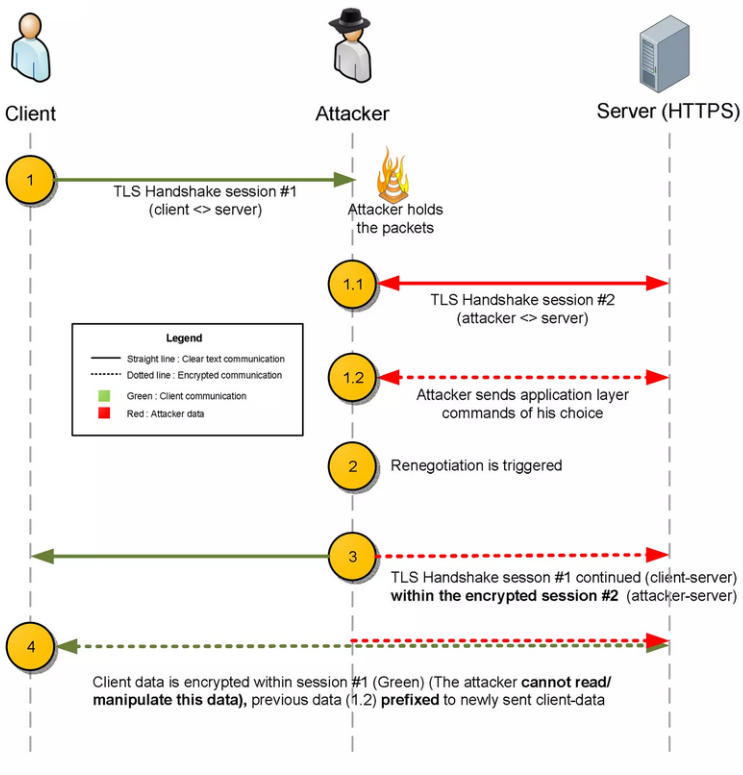
\includegraphics[scale=0.35]{../IMAGES/renegotiation.png}
        \label{regenetiation_attack}
    \end{figure}

    Вразливість преузгодження SSL - це вразливість, що дозволяє переузгоджувати SSL сесію на правах зловмискика так, що він таким чином може надсилати свої команди від імені клієнта.

    
    Вразливість переузгодження SSL в першу чергу впливала на протоколи SSL/TLS до версії TLS 1.2, включаючи SSL 3.0 і TLS 1.0, а також деякі реалізації TLS 1.1.


    Ця атака діяла таким чином як показано на картинці \ref{regenetiation_attack}. Самою суттю є перехоплення трафіку на початку зловмисником та формування, а саме в атаці зловмисник використовує процес переузгодження SSL сесії, щоб вставити шкідливі дані в поточний сеанс SSL. Процес починається, коли зловмисник перехоплює початкове повідомлення <<Client Hello>> від клієнта до сервера. Встановивши SSL-з'єднання з сервером за допомогою цього перехопленого повідомлення, зловмисник може запросити сервер на повторне узгодження.


    Під час цього перегляду зловмисник пересилає оригінальне повідомлення <<Client Hello>> від клієнта до сервера. Сервер, вважаючи, що він веде переговори з початковим клієнтом, продовжує процес рукостискання. Тим часом, клієнт думає, що він встановлює нову сесію. Ця невідповідність дозволяє зловмиснику перехоплювати і маніпулювати захищеним зв'язком між клієнтом і сервером, фактично перехоплюючи сеанс.

    
\item \textbf{Атака відкату версії}

    Атаки відкату версії використовують переваги зворотної сумісності системи, щоб перевести її в менш безпечні режими роботи. До прикладу, під час атаки на пониження версії HTTPS відвідувачі вашого веб-сайту можуть бути змушені використовувати з’єднання HTTP замість HTTPS. Атака зниження версії може бути невеликою частиною більшої зловмисної операції. Така атака є можливою завдяки властивостям зворотньої сумісності системи.


\item \textbf{SSL strip}

    sslstrip - це назва атаки, що була проведена Моксі Марлінспайк у 2009 році на конференції Black Hat. У загальному ця атака використовувала відсутність примусового застосування HTTPS на багатьох веб-сайтах шляхом перехоплення та зниження рівня HTTPS до HTTP, дозволяючи нападникам маніпулювати чутливими даними, що передаються мережею.

    Ця атака могла бути проведеною точно так само як на картинці \ref{ssl_strip}.

\begin{figure}[ht]
        \centering
        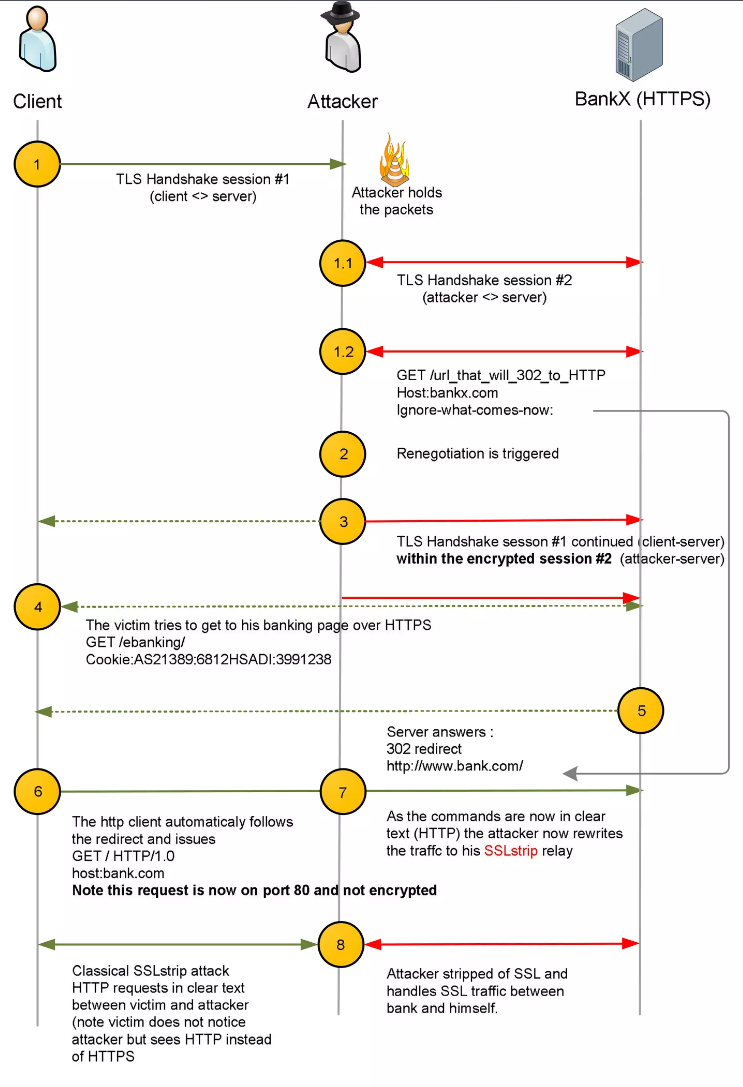
\includegraphics[scale=0.35]{../IMAGES/ssl_strip.png}
        \label{ssl_strip}
\end{figure}

    Суть атаки полягала у тому, що раніше браузери не були такими розвиненими та вони всіляко опиралися щодо вводу більш явних значків безпеки на сайтах:
\begin{enumerate}
    \item Раніше значки замочка (сигналізує використання HTTPS) не були такими яскравими і явними. Вони всі були однотонні і не давали користувачу уявлення, що щось іде не так.
    \item Саме на той час уже з'явився HTTPS протокол, але всі переходити на нього не спішили, тому був введений проміжний варіант, де користувач переходив лише на сторінку HTTP, а лише потім при авторизації спеціальна кнопка переводила користувача у захищений режим HTTPS. 
\end{enumerate}


    Тобто у результаті зловмисник уже знав, що на конкретному сайті буде такий запит і міг слухати трафік та лише за необхідності зробити свою сесію разом із якою він буде перенаправляти трафік жертві. При цьому жертва не побачить жодним чином, що перехід на захищену версію сайта не відбувся лише по маленьким буквам у адресному рядку.


    Також додамо, що ця атака мала один мінус, а саме те, що не було можливим понизити існуючу SSL сесію і вона могла працювати лише за умови, що користувач отримує доступ до банку спершу через HTTP, а потім пробує перевести свої чутливі дані до HTTPS.


\item \textbf{Атаки на шифр RC4}
    RC4 - це потоковий шифр, який широко використовується для безпечного зв’язку, зокрема в таких протоколах, як SSL/TLS і WEP. Він став відомий своєю швидкістю та простотою, але з часом були виявлені вразливості, що послабило його надійність у безпечному зв’язку. У 2015 році близько 30\% трафіку було зашифровано ним.


    Загалом відповідно до FMS дослідження було виявлено 2 значущі вразливості:
    \begin{itemize}
        \item вхідного вектора (IV), що призвело до практичної атаки відновлення ключа та повного зламування RC4 у протоколі WEP;
        \item інваріантності, що залишалася невідомою 13 років (або Invariance Weakness).
    \end{itemize}

    
    Остання вразливість була використана у атаці Bar Mitzvah, що веде до відновлення захищених кешованих даних, повідомлень після збирання трафіку для статистичної обробки.

    \begin{figure}[!ht]
        \centering
        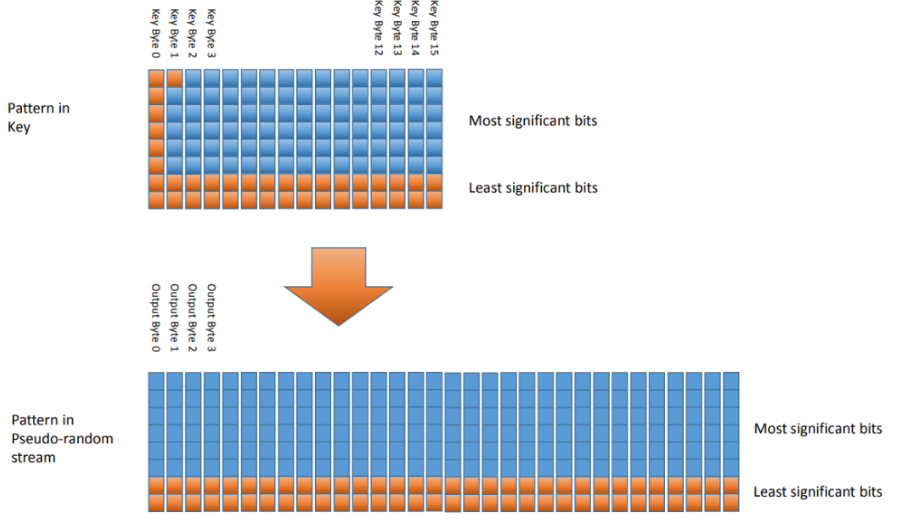
\includegraphics[scale=0.35]{../IMAGES/rc4_l_pattern.png}
        \label{weak_keys_rc4}
    \end{figure}

    Вона базувалася на використанні слабких ключів, що дозволяли відновити молодші біти байтів відкритого тексту. Invariance Weakness базується на нявності L-подібного шаблону ключа в ключах RC4, який зберігає перестановку станів та зберігає частину перестановки станів недоторканою протягом усього процесу ініціалізації. Ця незмінна частина включає молодші біти перестановки при обробці алгоритмом псевдо-випадкового генератора (PRGA), визначає молодші біти нібито псевдовипадкового вихідного потоку за довгим префіксом потоку. Ці викривлені байти потоку додаються до байт відкритого тексту за допомогою операції XOR, що призводить до значного витоку байт відкритого тексту з байт зашифрованого тексту.
    
    \item \textbf{Атаки на генератор псевдовипадкових чисел}

    У TLS документації є згадки про псевдовипадкову функцію (PRF або Pseudo random function), що обсислює HMAC для генерування значень. Більшість атак на PRF зводиться до атаки на геш функцію, а саме пошук колізій у них. До прикладу, TLS 1.1 PRF базується на комбінації MD5 і SHA-1. І MD5, і SHA-1, що не дають впевненості у цьому генераторі, адже ці геш-функції були нестійкими до колізій. У пізніших версіях TLS 1.2 та 1.3 замінюють ці геш функції на SHA-256 та SHA-384.

    \item \textbf{POODLE}

    POODLE (або Padding Oracle On Downgraded Legacy Encryption) — ця атака дозволяє зловмиснику, наприклад зловмисній точці доступу Wi-Fi або скомпрометованому інтернет-провайдеру, отримувати дані з HTTPS-з’єднань. Це, у свою чергу, може дозволити зловмиснику отримати доступ до онлайн-банкінгу або системи електронної пошти. 


    Атака реалізується лише на SSL 3.0. Недоліком SSL 3.0 є досконала не перевіряє певні частини даних, які супроводжують кожне повідомлення. Зловмисники можуть використовувати цю слабкість, щоб розшифрувати окремий байт і час зашифрованих даних, таким чином можна побайтно витягувати звичайний текст повідомлення.


    Найбільш вразливою програмою є HTTP. Приклад сценарію атаки спрацював би приблизно такий. Зловмисник встановлює шкідливу точку доступу Wi-Fi. Ця точка доступу Wi-Fi виконує дві функції. Під час незахищених HTTP-з’єднань він вставляє фрагмент JavaScript. А в захищених HTTP-з’єднаннях він перехоплює вихідні повідомлення та реорганізує їх. Метою зловмисника є отримання файлу cookie сеансу HTTP, який використовується над певним зацікавленою сторінкою, до прикладу, веб-пошта. За допомогою цього файлу cookie сеансу зловмисник може отримати доступ до поштової служби, видаючи себе за жертву. Впроваджений Меллорі JavaScript повідомляє браузеру кілька разів спробувати завантажити зображення з цієї веб-пошти. Кожен запит зображення містить файл cookie сеансу, і JavaScript гарантує, що кожен із цих запитів створено таким чином, щоб один байт файлу cookie сеансу розміщувався в певному місці в кожному SSL-повідомленні.

    
    TLS 1.0 і новіші версії виконують більш надійну перевірку розшифрованих даних і тому не схильні до такої ж проблеми.
    
    \item \textbf{Атака BEAST}

    Атака BEAST (або Browser Exploit Against SSL/TLS) (BEAST) була розкрита у вересні 2011 року. Вона стосується SSL 3.0 і TLS 1.0, тому впливає на браузери, які підтримують протоколи TLS 1.0 або раніші. Зловмисник може розшифрувати дані, якими обмінюються дві сторони, скориставшись уразливістю в реалізації режиму з’єднання шифрованих блоків (CBC) у TLS 1.0.


    Зловмисник використовує man-in-the-middle для введення пакетів у потік TLS. Це дозволяє зловмисникам вгадати вектор ініціалізації, що використовується з введеним повідомленням, а потім просто порівняти результати з результатами блоку, який вони хочуть розшифрувати.


    Щоб атака BEAST була успішною, зловмисник повинен мати певний контроль над браузером жертви. Таким чином, зловмисник може вибрати легший вектор атаки замість цього.
    
    
    
    \item \textbf{CRIME}

    Вразливість CRIME (або Compression Ratio Info-leak Made Easy) впливає на стиснення TLS. Вибір методу стиснення включено в повідомлення Client Hello і є необов’язковим. Стиснення було введено в SSL/TLS, щоб зменшити кількість інформації, якою обмінюються абоненти.


    Припустимо, зловмисник хоче отримати секретний cookie жертви. Зловмисник заздалегідь знає, що цільовий веб-сайт (examplebank.com) створює файл cookie для сеансу. Він, спостерігає за зміною розміру стисненого корисного навантаження запиту, що містить як секретний файл cookie, який надсилається жетвою лише на сервер, так і змінюваний зміст створений зловмисником. При передачі повідомлення наш трафік буде стискатися, а відповідно як розмір стисненого вмісту зменшується, то можна зробити висновок, що існує ймовірність того, що деяка частина частково зміненого вмісту міститься у секретному файлі. У результаті зловмисник буде намагатися відновити цілий файл із cookie.

    \begin{figure}[ht]
        \centering
        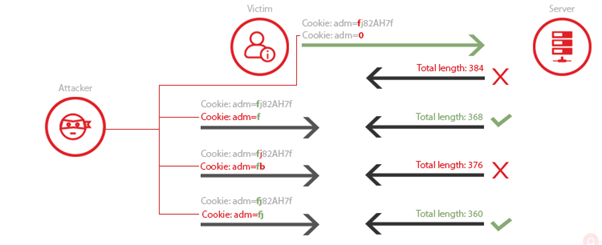
\includegraphics[scale=0.35]{../IMAGES/crime_2.png}
        \label{weak_keys_rc4}
    \end{figure}

    
    \item \textbf{BREACH}
    Вразливість BREACH (або Browser Reconnaissance and Exfiltration via Adaptive Compression of Hypertext) дуже схожа на CRIME, але BREACH спрямована на стиснення HTTP, а не на TLS. Ця атака можлива, навіть якщо стиснення TLS вимкнено. Зловмисник змушує браузер жертви підключатися до стороннього веб-сайту з підтримкою TLS і відстежує трафік між жертвою та сервером за допомогою атаки man-in-the-middle.

    
    \item \textbf{FREAK}

    Атака FREAK (або Factoring RSA Export Keys) є атакою на дивне обмеження NSA на ключі, що могли використовуватися при експорті додатків із території США. У зв'язку із тим, що у ті часи було популярно використовувати RSA, разом із перехопленням трафіку можна було штучно перевести користувача на експорту версію алгоритма із 512 бітними ключами, що у 2010-ті можна було уже перебрати за 1 годину використовуючи ефективні алгоритми факторизації. Тож разом із цим зловмиснику було легко дізнатися pre-master-secret, а разом із ним і всі інші сеансові ключі.
    
    \item \textbf{Logjam}

    Саме тут використовуються точно так сама ідея із експортними алогритмами із США, але тільки усе іде для замішування ключів за допомогою Діффі-Геллмана. Експртний варіант систем побудованих на даному ключовому обміні повинен мати бітність рівну 512.
    
    
    \item \textbf{Heartbleed}

    Дана вразливість скоріше є помилкою у реалізації, що давала можливість зловмисникам дізнаватися інформацію, що вони не повинні були знати за межами рамок довжини масиву байтів. Помилка була у імплементації розширення до TLS - heartbeat, що дозволяло серверу продовжувати комунікацію із клієнтом, знаючи що сесія ще не була розірвана. 

    
    Цей серйозний недолік полягає в перевірці відсутніх меж перед викликом memcpy(), який використовує необроблений введений користувачем параметр довжини. Зловмисник може обманом змусити OpenSSL виділити буфер розміром 64 КБ, скопіювати в буфер більше байтів, ніж необхідно, надіслати цей буфер назад і, таким чином, отримати витік вмісту пам’яті жертви, по 64 КБ за раз.

        
    
    \item \textbf{Атака BERserk}
    Ця вразливість дозволяє зловмисникам підробляти підписи RSA, таким чином дозволяючи обходити автентифікацію для веб-сайтів, які використовують TLS. Ця атака використовує вразливість у аналізі повідомлень, закодованих ASN.1 під час перевірки підпису. Повідомлення ASN.1 складаються з різних частин, які кодуються за допомогою BER та/або DER. Ця атака використовує той факт, що довжина поля в кодуванні BER може використовувати велику кількісь байтів даних. У вразливих реалізаціях ці байти пропускаються під час аналізу, що і дає простір для атаки.
    

    \item \textbf{ARP спуфінг}

    Протокол вирішення адреси (або ARP - Address Resolution Protocol) - це комунікаційний протокол, що використовуєтья для виявлення адреси канального рівня, до прикладу MAC адреси. Тобто у зв'язку із тим, що більшість комп’ютерних програм/додатків використовують логічні адреси (IP-адреси) для надсилання/отримання повідомлень. Однак фактичний зв’язок відбувається через фізичну адресу (MAC-адресу) із рівня 2 моделі OSI. Тому наша місія полягає в тому, щоб отримати MAC-адресу, що допоможе спілкуватися з іншими пристроями. 


    Сама підміна ARP може відбутися на LAN рівні. Атака відбувається таким чином, що користувач А знає, що у хоста Б будуть всі відповідні адреси у розпорядженні і потрібний запит надійде по правильному шляху. Зловмисник у свою чергу знає цей факт і намагається переконати кристувача А, що саме він є хостом Б, хоча насправді є хостом $\text{Б}^{'}$. Таким чином кожного разу як користувач А, думає, що він спілкується із користувачем Б, насправді відправляє увесь свій трафік через хост $\text{Б}^{'}$, що його прослуховує і може вільно модифікувати повідомлення, що проходять через нього.


    Ціллю атаки ARP підміни є шпигунство, або атаки типу "man-in-the-middle" або для додаткових кібератак, до прикладу, <<denial of service>>.
    
\end{itemize}


\subsection{Рекомендації для використання протоколу TLS}

\begin{itemize}
    \item \textbf{Оновлюйте версію TLS}


    Використовуйте найновішу версію TLS, оскільки нові версії пропонують покращення фукнції безпеки порівняно зі старими протоколами, які є вразливими до різного роду атак.
    
    \item \textbf{Використовуйте надійний центр сертифікації}


    Ваші сертифікати такі ж надійні як і ЦС, що їх видає, тож їх треба вчасно оновлювати та використовувати надійні алгоритми.
    
    \item \textbf{Впровадження HSTS}


    HTTP Strict Transport Security (HSTS) — це механізм політики безпеки, який допомагає захистити веб-сайти від атак із пониженням версії протоколу та викрадення файлів cookie. Він дозволяє веб-серверам декларувати, що веб-браузери (або інші відповідні агенти користувача) повинні взаємодіяти з ним лише за допомогою безпечних з’єднань HTTPS, а не через незахищений протокол HTTP.
    
\end{itemize}